\chapter{Numerical Differentiation and Integration}
\section{Differentiation}

\begin{thm} [Two Points Formula]
	\begin{align*}
	f'(x_0) &= \frac{f(x_0 + h) - f(x_0)}{h} - \frac{h}{2} f''(\zeta),\;\text{forward difference} \\
	f'(x_0) &= \frac{f(x_0 - h) - f(x_0)}{-h} + \frac{h}{2} f''(\zeta),\;\ \text{backward difference}
	\end{align*}
\end{thm}
\begin{proof}
	Suppose we are given two data points $(x_0,f(x_0))$ and $(x_0+h,f(x_0+h))$. We first start with Lagrange interpolation,
	\[ f(x) = f(x_0)\frac{x-x_0-h}{-h} + f(x_0+h)\frac{x-x_0}{h} + \frac{(x-x_0)(x-x_0-h)}{2}f''(\zeta) \]
	where $\zeta\in[x_0,x_0+h]$ is number such that $f''$ is maximized. Thus the differentiation of this gives us
	\begin{align*}
	f'(x) &= f(x_0)\frac{1}{-h} + f(x_0+h)\frac{1}{h} + \frac{d}{dx}\left[ \frac{(x-x_0)(x-x_0-h)}{2}f''(\zeta) \right]\\
	&= \frac{f(x_0+h)-f(x_0)}{h} + \frac{2(x-x_0)-h}{2}f''(\zeta) + \frac{(x-x_0)(x-x_0-h)}{2}\frac{d}{dx}f''(\zeta)\\
	\end{align*}
	When $x=x_0$, then we have
	\[ f'(x_0) = \frac{f(x_0+h)-f(x_0)}{h} - \frac{h}{2}f''(\zeta)\]
\end{proof}

You need to know this derivation of two point formula (including the error term).

\begin{thm} [Three Points Formula]
	\begin{align*}
	f'(x_0) &= \frac{1}{2h} (-3f(x_0) + 4f(x_0+h) - f(x_0+2h))  - \frac{h^2}{3}f'''(\zeta), \; \text{Left end point}\\
	f'(x_0) &= \frac{1}{-2h} (-3f(x_0) + 4f(x_0-h) - f(x_0-2h))  - \frac{h^2}{3}f'''(\zeta), \; \text{Right end point}\\
	f'(x_0) &= \frac{1}{2h} (f(x_0+h) - f(x_0-h))  - \frac{h^2}{6}f'''(\zeta), \; \text{Mid point}
	\end{align*}
	
\end{thm}


\begin{thm} [Three points formula for second derivative]
\[ f''(x_0) = \frac{1}{h^2} (f(x_0-h) - 2f(x_0) + f(x_0+h) )- \frac{h^2}{12} f^{(4)}(\zeta)\]
\end{thm}


\section{Integration}
\begin{thm} [Trapozoidal rule]
	\[\int_{x_0}^{x_1} f(x)dx = \frac{h}{2} (f(x_0) + f(x_1)) - \frac{h^3}{12} f''(\zeta)\]
\end{thm}

\begin{thm} [Simpson's rule]
	\[\int_{x_0}^{x_2} f(x)dx = \frac{h}{3} (f(x_0) + 4f(x_1) + f(x_2))- \frac{h^5}{90} f^{(5)}(\zeta)\]
\end{thm}

\begin{thm} [Composite Trapozoidal rule]
\[ \int_{x_0}^{x_n} f(x)dx = \frac{h}{2}\left ( f(x_0) + 2\sum_{i=1}^{n-1}f(x_i) + f(x_n) \right ) - \frac{x_n-x_0}{12}h^2 f'''(\zeta)\]
\end{thm}

\begin{thm} [Composite Simpson's rule]
	\[ \int_{x_0}^{x_n} f(x)dx = \frac{h}{3}\left ( f(x_0) + 4\sum_{k=1}^{n/2}f(x_{2k-1}) + 2\sum_{k=1}^{n/2-1}f(x_{2k}) +f(x_n) \right ) - \frac{x_n-x_0}{180}h^4f^{(4)}(\zeta) \]
\end{thm}

\begin{thm} [Adaptive Quadrature]
	Suppose we want to approximate $\int_a^b f(x)dx$ within some tolerance $\epsilon$, then we can achieve that by increasing the number of partitions.
	\[\left|\int_a^bf(x)dx - S(a,b)\right|
	\geq \left|\int_a^bf(x)dx - S\left(a,\frac{a+b}{2}\right) - S\left(\frac{a+b}{2}, b\right)\right| \]
	where $S$ stands for Simpsons' rule. And the estimation of error is given by
	\begin{align*}
	&\left|\int_a^bf(x)dx - S\left(a,\frac{a+b}{2}\right) - S\left(\frac{a+b}{2}, b\right) \right|\\ 
	&\approx 
	\frac{1}{15}\left|S(a,b) - S\left(a,\frac{a+b}{2}\right) - S\left(\frac{a+b}{2}, b\right)\right|
	\end{align*}
	There is a factor $1/15$ because we are using Simpson's rule
\end{thm}

\begin{ex}
	Apply adaptive quadrature once to approximate the integral and estimate its error
	\[ \int_0^{\frac{\pi}{2}} \sin xdx \]
	\begin{solution}
		Apply adaptive quadrature once, we have
		\begin{align*}
		\int_0^{\frac{\pi}{2}} \sin xdx 
		&\approx S\left(0,\frac{\pi}{4}\right) + S\left(\frac{\pi}{4}, \frac{\pi}{2}\right)\\
		&= \frac{\pi/8}{3}\left[ \sin 0  + 4\sin \frac{\pi}{8} + 2\sin \frac{\pi}{4} + 4\sin \frac{3\pi}{8} + \sin\frac{\pi}{2} \right]\\
		&= 1.000134585
		\end{align*}
		
		On the other hand, since
		\[ S\left(0,\frac{\pi}{2}\right) = \frac{\pi/4}{3}\left[ \sin 0 + 4\sin \frac{\pi}{4} + \sin\frac{\pi}{2} \right] = 1.002279878 \]
		
		We have 
		\begin{align*}
		&\left|\int_0^{\frac{\pi}{2}}\sin xdx - S\left(0,\frac{\pi}{4}\right) - S\left(\frac{\pi}{4}, \frac{\pi}{2}\right)\right| \\
		&\approx 
		\frac{1}{15}\left|S(a,b) - S\left(a,\frac{a+b}{2}\right) - S\left(\frac{a+b}{2}, b\right)\right|
		&= 0.000143020
		\end{align*}
		
		If we do this integral by hand, we see that the actual error is 
		\[ \left| \int_0^{\frac{\pi}{2}}\sin xdx - 1.000134585 \right| = \left| 1 - 1.000134585 \right| = 0.000134585 \]
		We see that the estimated error is very close to the actual one.
	\end{solution}
\end{ex}


\begin{summary}
	Few things about  adaptive quadrature worth to mention.
	\begin{enumerate}
		\item You only need to increase partition in the subinterval where it fails the tolerance! 
		\item Adaptive quadrature can be adapted to other numeric integration rules.
		\item This technique does not rely on higher derivatives of the function.
	\end{enumerate}
\end{summary}

\begin{thm} [Gaussian quadrature]
	\[\int_{-1}^{1} f(x)dx = \sum_{j=1}^n c_{n,j}f(r_{n,j}) \]
	
	where $r_{n,j}$ is the jth root of nth Legendre polynomial, and $c_{n,j}$ are the coefficients correspond to them.
	\begin{figure} [H]
		\centering
		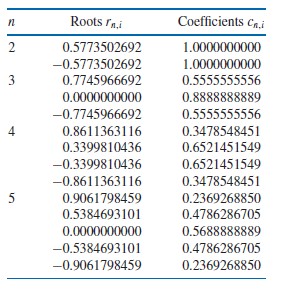
\includegraphics{img/zeros_legendre_p} 
	\end{figure}
	
	If the integration interval is $[a,b]$, then
	\[\int_{a}^{b} f(x)dx = \int_{-1}^{1} f\left(\frac{(b-a)t+ (b+a)}{2}\right) \frac{b-a}{2}dt = \frac{b-a}{2} \sum_{j=1}^n c_{n,j}f\left( \frac{(b-a)r_{n,j}+ (b+a)}{2} \right)
	\]
\end{thm}

\begin{ex}
	Approximate the integral using Gaussian quadrature with $n=3$.
	\[ \int_{-1}^1 e^x\cos xdx \]
	\begin{solution}
		\begin{align*}
		\int_{-1}^1 e^x\cos xdx &\approx 0.\bar{5}e^{0.774596692}\cos 0.774596692\\
		&+ 0.\bar{8}e^0\cos 0 + 0.\bar{5}e^{-0.774596692}\cos(-0.774596692)\\
		&= 1.9333904. 
		\end{align*}
		
		Integration by parts can be used to show that the true value of the integral is $1.9334214$, so the absolute error is less than $3.2\times 10^{-5}$.
	\end{solution}
\end{ex}

\begin{ex}
	Approximate the integral using Gaussian quadrature with $n=3$.
	\[ \int_{1}^3 x^6 - x^2\sin(2x)dx \]
	\begin{solution}
		Notice that this interval is $[1,3]$, so we need to change the variable $x\to t+2$. Thus, the integrand becomes
		\begin{align*}
		\int_{1}^3 x^6 - x^2\sin(2x)dx &= \int_{-1}^{1} f(t+2) dt\\
		&= 0.\bar{5}f(0.7745966692 + 2) \\
		&\phantom{=}+ 0.8f(0+2)\\
		&\phantom{=}+ 0.\bar{5}f(-0.7745966692 + 2)\\
		&= 317.2641516
		\end{align*}
	\end{solution}
\end{ex}

